% Created 2021-04-04 Sun 22:43
% Intended LaTeX compiler: pdflatex
\documentclass[11pt]{article}
\usepackage[utf8]{inputenc}
\usepackage[T1]{fontenc}
\usepackage{graphicx}
\usepackage{grffile}
\usepackage{longtable}
\usepackage{wrapfig}
\usepackage{rotating}
\usepackage[normalem]{ulem}
\usepackage{amsmath}
\usepackage{textcomp}
\usepackage{amssymb}
\usepackage{capt-of}
\usepackage{hyperref}
\usepackage{minted}
\usepackage[margin=1in]{geometry}
\usepackage{subcaption}
\author{A. Bochkarev}
\date{}
\title{Facility Location with BDDs: Status update 2}
\hypersetup{
 pdfauthor={A. Bochkarev},
 pdftitle={Facility Location with BDDs: Status update 2},
 pdfkeywords={},
 pdfsubject={},
 pdfcreator={Emacs 28.0.50 (Org mode 9.4.3)}, 
 pdflang={English}}
\begin{document}

\maketitle

\section{Status}
\label{sec:orgf8c8d9f}
\begin{itemize}
\item we are dealing with the Facility location problem in the following edition: every facility can
"cover" all its neighbors, we have to cover every customer at least once, no
overlap costs; we have "colored" facilities + budget for number of locations
per color.
\item I have implemented constructing BDDs for (1) \textbf{cover} constraints, and (2) \textbf{color} constraints.
\item with this problem formulation, intersection BDD is still very large, but now
we have at least something to discuss, as the process depends on many factors.
\item runtimes, to me, still do not look competitive with MIP -- we might want to
look into some specific instance types?
\end{itemize}

\section{The problem.}
\label{sec:org2728a9d}
First, let me re-introduce my ``model'' problem. Assume I have the following
seven nodes (costs are in the parentheses) of graph \(G\):
\begin{center}
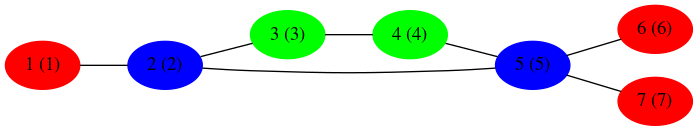
\includegraphics[width=.9\linewidth]{problem_LR.png}
\end{center}

Color limits are as follows: red (5), blue (1), green (3). (So, the point is: I
can't have two ``central'' blue nodes, \textcircled{2} and \textcircled{5}, at the
same time -- other limits are not binding.)

\section{Plan of attack}
\label{sec:org52d8665}
\begin{itemize}
\item build \textbf{cover} BDD (encode the condition ``every facility has to be covered at least once'');
\item build \textbf{color} BDD (encode the condition ``respect color budgets'');
\item make them order-associated;
\item build an intersection DD.
\item formulate and solve the network flow out of the intersection DD.
\end{itemize}

All of these steps are implemented now.

\section{Building the cover DD}
\label{sec:orga273f85}
\begin{itemize}
\item I keep track of a "state" -- a boolean vector of length \(N\) (number of nodes
in \(G\)) , denoting whether each node was covered or not. So, I have a
"covering" \emph{state} associated with every BDD node.
\item so, "incorporating" node (of \(G\)) to the BDD is straightforward: I just update
the states for all nodes adjacent to this "new" node, with the following caveat.
\item if from some state there is no way I could cover at least one node (of \(G\))
further, I connect the respective BDD node to the ``trash pipe'' (a set of
nodes with no path to \textbf{True} terminal).
\item to keep track of such "opportunities further in the BDD", I basically keep the
remaining \emph{"freedoms"} of \(G\) nodes: node degree minus the number of its
neighbors already present in the diagram above. When such number drops to
zero, then there is no way the "state" of the node ("covered" vs. "not
covered" can be changed further down the BDD).
\item so, I "process" nodes one by one as follows. I just "incorporate" the node,
and then all its neighbors, into the BDD. For example, "processing" node
\textcircled{1} involves incorporating nodes \textcircled{1} and
\textcircled{2}. Processing \textcircled{2} would involve incorporating
\textcircled{1}, \textcircled{2}, \textcircled{3}, and \textcircled{5}, and so
on.
\item Again, after every node processing I update the node "freedoms".
\item I take special care of the nodes which "freedoms" has just dropped to zero: the ones
that are not covered will drive the respective BDD state (BDD node) to the
``trash pipe''.
\item The final piece of the puzzle is the order of nodes processing. I just pick
the node with the smallest number of "freedoms" every time.
\item edge weights are zeroes, except for "yes"-arcs for non-trash-sleeve nodes,
where the weights correspond to location costs.

The resulting diagram for the problem above presented in Figure \ref{fig:cover}.
\end{itemize}

\begin{figure}[htbp]
\centering
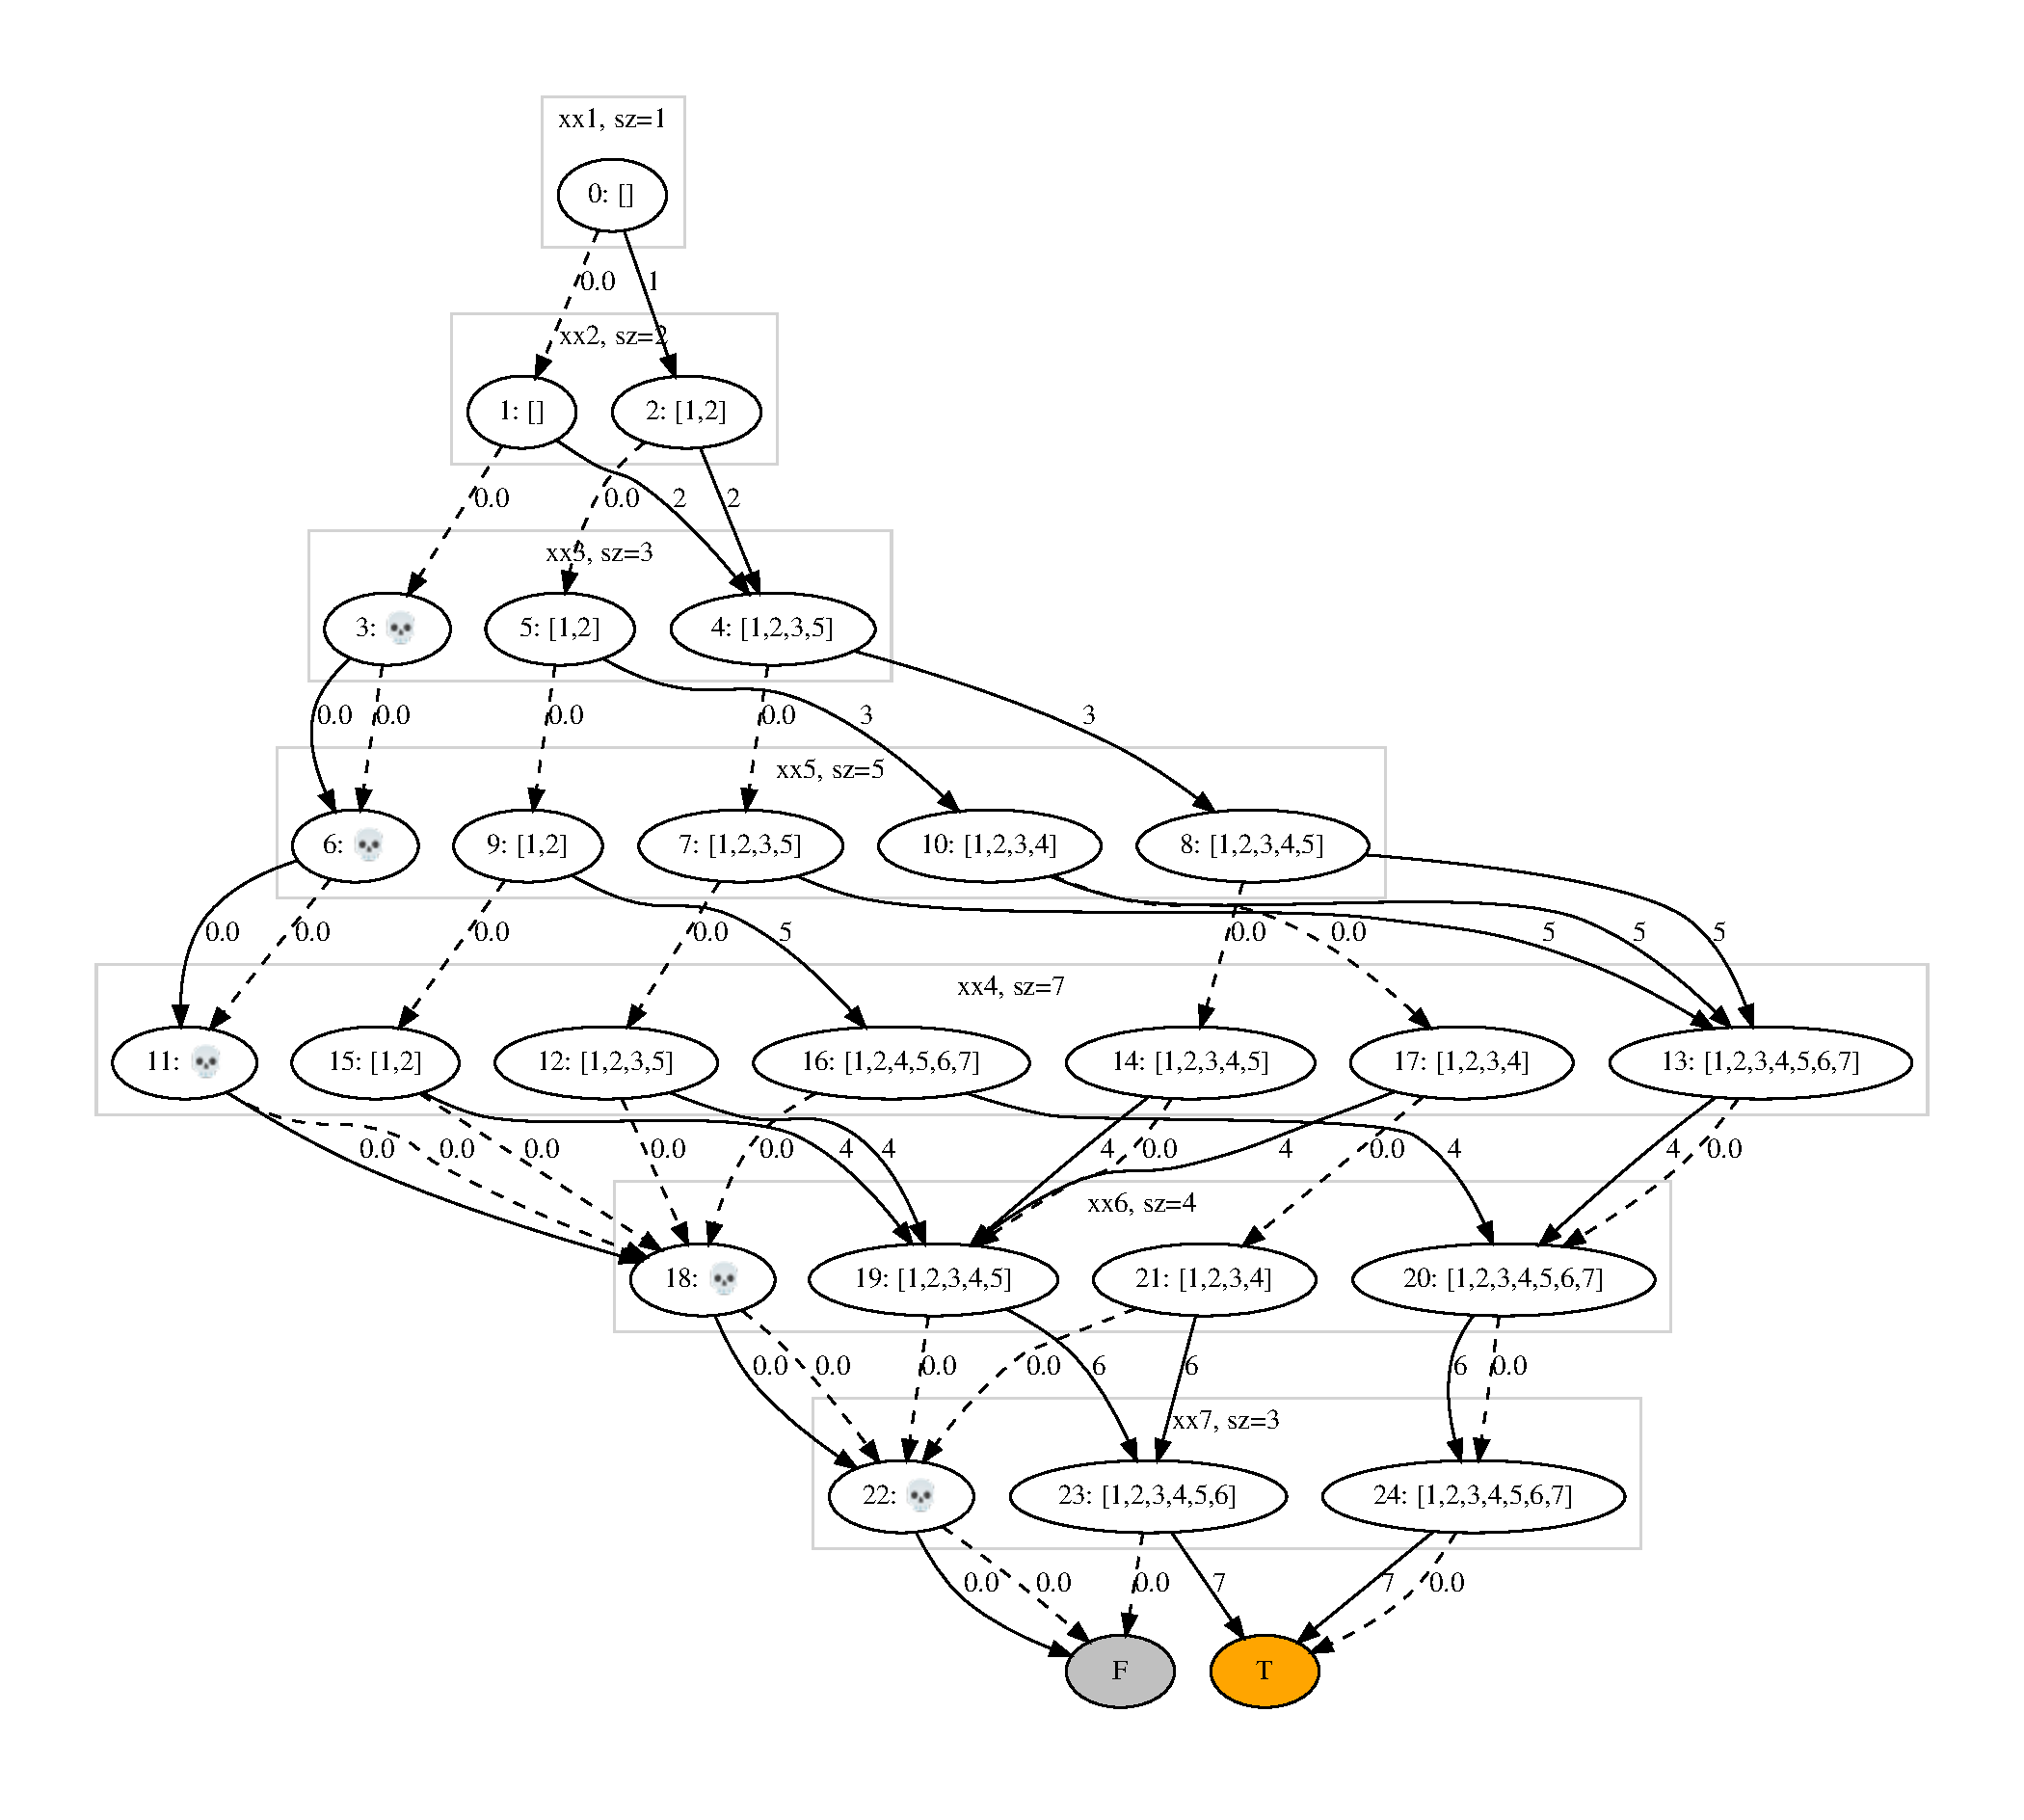
\includegraphics[width=530px]{./cover.png}
\caption{\label{fig:cover}The \textbf{cover} diagram (numbers in \texttt{[brackets]} are nodes covered in the respective state; ``trash sleeve'' is denoted by skulls). I start with \textcircled{1}, adding layers for \textcircled{1} and \textcircled{2}. Note that \textcircled{3} has 3 freedoms now (depending on \textcircled{2}, \textcircled{3}, and \textcircled{4}). The next node to process will be one with the minimal freedoms -- either \textcircled{6} or \textcircled{7} (each with two). So \textcircled{6} and \textcircled{5} are added, and so on.}
\end{figure}

\section{Building the color DD}
\label{sec:org98db2f4}
\begin{itemize}
\item building the \textbf{color} diagram is simple: I would need to pick an \emph{order} for
colors, and then, within each color the state is number of locations already
"used". For example, if the budget for green is 3 locations, I might have
states up to \{\texttt{0}, \texttt{1}, \texttt{2}, \texttt{3}, and \texttt{(infeasible)}\} in any ``green'' layer
of the color diagram.
\item of course, after every color block the layer width is reset to at most two
(comprising state \texttt{0} and, perhaps, \texttt{(infeasible)}).
\item now, ordering does matter, of course, and we have certain flexibility here: I
can pick any order \emph{within} each color, and I can arbitrarily shuffle
\emph{colors}. So, what I am doing is:
\begin{itemize}
\item \emph{within} each color order of \(G\) nodes correspond to their relative order in the cover diagram.
\item \emph{between} colors\ldots{} Well, I move colors around (as blocks) in a procedure
\textbf{very} similar to a bubble sort.\footnote{oh, this is a strange story. I can ``compare'' any two colors \(C_1\)
and \(C_2\) (relative to the target order of nodes in \(G\)), in the sense that I
can say, what gives me more inversions with the cover diagram: \(C_1 \prec C_2\)
or \(C_2 \prec C_1\). The only thing is: I am not sure the resulting relation is
transitive\ldots{} And so, perhaps, every 300th or 400th random example is off by
1--2 inversions from the optimum. Anyways, the way I have implemented it now
allowed to cut no. of nodes and runtimes approx. 2--3 times, I think, compared
to the trivial ordering (1, 2, 3, \(\ldots\)).}
\end{itemize}
\item in fact, I did not use any weights in this diagram (all are zeroes).
\end{itemize}

The resulting diagram for the problem above looks as presented in Figure \ref{fig:color}.

\begin{figure}[htbp]
\centering
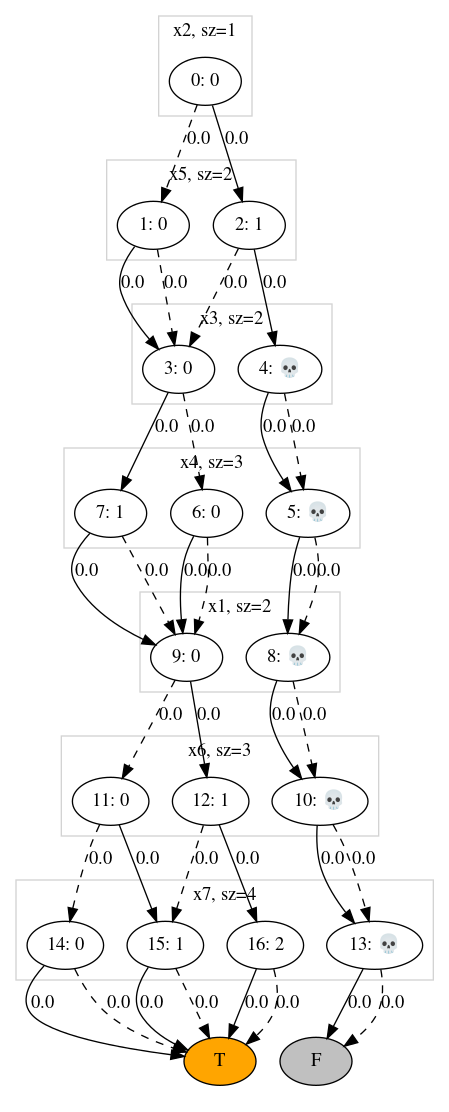
\includegraphics[width=250px]{./color.png}
\caption{\label{fig:color}The \textbf{color} diagram. The order of colors is: blue (\textcircled{2}, \textcircled{5}) -- green (\textcircled{3}, \textcircled{4}) -- red (\textcircled{1}, \textcircled{6}, \textcircled{7}).}
\end{figure}

\section{The intersection DD.}
\label{sec:orgb78f4bd}
The procedure is (conceptually) simple: a "state" is now defined by a pair of
node IDs. For example, if I intersect diagrams \(D_1\) and \(D_2\), considering
nodes \(u\in D_1\) and \(v\in D_2\), the intersection diagram will have the
following two nodes in the next layer: \((1(u), 1(v)\) and \((0(u), 0(v))\) (where
\(1(a)\) denotes a head of one arc emanating from \(a\), and \(0(a)\) --
respectively, for a zero arc).

So, we have the following statistics for the number of nodes for our
particular example (excluding the two terminal nodes):
\begin{verbatim}
BEFORE the alignment:
cover size: 25, color size: 17
AFTER the alignment:
cover size: 26, color size: 18
intersection size: 38 nodes
\end{verbatim}


An intersection DD, of course, allows to build a network flow problem (which is
an LP, albeit in a large network) -- neither the idea, nor the code are new.

\section{Some results of numerical modeling.}
\label{sec:org3c267b8}

\subsection{Diagram sizes (table)}
\label{sec:org2ef2e7c}
Let me provide a raw table for the diagram sizes in some random experiments --
see Listing \ref{fig:sizes}. To me, this table highlights the key problem I am having
at the moment. I have also run some experiments to benchmark BDD-based methods
with this "plain MIP": of course, given the intersection sizes, for \(n=30\) nodes
in \(G\) I have the intersection-based thing 1--3 orders of magnitude slower than
the plain the MIP. It is still as bad as replacing a complicated-type problem
with 40-ish variables and constraints with a simple-type problem with, like,
40k-ish variables\ldots{} (and I do not think it behaves well asymptotically, as the size grows\ldots{})

\begin{listing}[htbp]
\begin{minted}[frame=lines,fontsize=\scriptsize,xleftmargin=\parindent,linenos]{text}
Raw data: numerical experiment 1 (2020-04-02)
    
                                          |          Plain MIP             | Experiment
n |size(color)|size(cover)| Intersection  | No. of vars   | No. of constr. | time (sec.)
--+-----------+-----------+---------------+---------------+----------------+-------------
5 | 9         | 10        | 14            | 5             | 8              | 0.0
5 | 6         | 11        | 13            | 5             | 9              | 0.0
5 | 7         | 11        | 12            | 5             | 8              | 0.0
5 | 7         | 11        | 18            | 5             | 8              | 0.0
5 | 9         | 14        | 20            | 5             | 7              | 0.0
7 | 10        | 18        | 24            | 7             | 12             | 0.0
7 | 14        | 19        | 30            | 7             | 10             | 0.0
7 | 18        | 22        | 41            | 7             | 9              | 0.0
7 | 11        | 27        | 33            | 7             | 11             | 0.0
7 | 10        | 22        | 33            | 7             | 12             | 0.0
10| 32        | 71        | 130           | 10            | 12             | 0.0
10| 23        | 46        | 73            | 10            | 14             | 0.0
10| 27        | 60        | 128           | 10            | 14             | 0.0
10| 11        | 60        | 60            | 10            | 19             | 0.0
10| 31        | 43        | 121           | 10            | 13             | 0.0
15| 31        | 411       | 633           | 15            | 21             | 0.1
15| 70        | 256       | 966           | 15            | 17             | 0.1
15| 33        | 146       | 262           | 15            | 23             | 0.1
15| 50        | 108       | 445           | 15            | 19             | 0.1
15| 48        | 156       | 587           | 15            | 20             | 0.1
20| 47        | 607       | 930           | 20            | 28             | 0.1
20| 54        | 3115      | 4481          | 20            | 28             | 1.0
20| 65        | 1756      | 4498          | 20            | 25             | 0.9
20| 84        | 2270      | 3953          | 20            | 22             | 0.8
20| 67        | 1689      | 3531          | 20            | 25             | 0.9
25| 122       | 10400     | 22658         | 25            | 27             | 4.0
25| 119       | 10281     | 22248         | 25            | 29             | 2.8
25| 82        | 5234      | 13295         | 25            | 29             | 3.1
25| 78        | 3320      | 9282          | 25            | 31             | 1.7
25| 104       | 6934      | 14346         | 25            | 28             | 2.7
30| 86        | 21872     | 24613         | 30            | 36             | 9.8
30| 103       | 24867     | 46515         | 30            | 39             | 13.2
30| 96        | 29752     | 44876         | 30            | 38             | 13.1
30| 119       | 35965     | 53781         | 30            | 36             | 17.7
30| 120       | 17616     | 51990         | 30            | 37             | 14.1
--+-----------+-----------+---------------+---------------+----------------+-------------
\end{minted}
\caption{\label{fig:sizes}Diagram sizes vs. number of variables and constraints in a plain MIP (depending on \(n\) -- number of nodes in \(G\), the original graph).}
\end{listing}

\section{Random instances generation}
\label{sec:org43b2e60}

\section{Discussion}
\label{sec:org114f8b6}
\begin{itemize}
\item sorting variables in \texttt{color} diagram.
\item random graph generation (limit node degree?)
\item next node selection in the (cover) BDD generation procedure.
\end{itemize}
\end{document}